\setchapterpreamble[u]{\margintoc}
\chapter{Methodology}~\label{chapter-methodology}

\epigraph{Is there method in the madness?}{Anon (1964--on)}
% \epigraph{I recall seeing a package to make quotes}{Snowball} %
% Uncommenting either of the epigraphs clashes somehow with the first figure in this chapter {fig:six-perspectives-in-the-methodology} and causes a cascading compilation error: You can't use `\prevdepth' in horizontal mode.
% Amazingly, the answer was to add a blank line before the epigraph command. See https://tex.stackexchange.com/a/569632/88466



The research was designed to address the main research question: \href{overall-research-question}{\emph{How can applying analytics improve software development and software testing for mobile apps in practice?}}\index{Research question}. The six perspectives introduced in the Introduction (on page~\pageref{rq-leads-to-six-perspectives}) and repeated here in Figure~\ref{fig:six-perspectives-in-the-methodology} for ease of reference direct attention to two key dimensions of investigation:
\begin{enumerate}
    \item the different \emph{objects of analysis}: the software development processes used by app developers, the software product (\emph{i.e.}, app) and related development artefacts, and the mobile analytics tools; 
    
    \item a \emph{temporal} dimension considering what \emph{is} (\emph{i.e.}, the current status) and what \emph{could be} (\emph{i.e.}, scope for improvements relating to the objects of analysis.
\end{enumerate}

\begin{figure*}
    \centering
    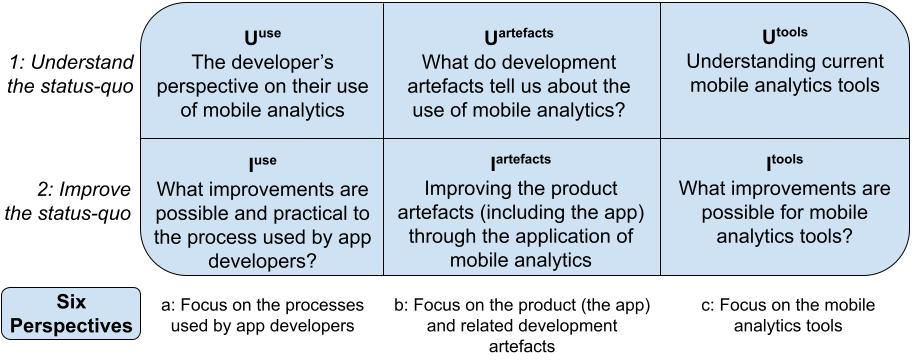
\includegraphics[width=\linewidth]{images/my/six-perspectives-2x3-matrix-12-nov-2021.jpeg}
    \caption{Methodology six perspectives (repeated)}
    \label{fig:six-perspectives-in-the-methodology}
\end{figure*}

The research is both \emph{knowledge-seeking} and \emph{solution-seeking} in nature~\sidecite[][p. 11-4]{stol2018_the_abc_of_software_engineering_research}. It is knowledge-seeking in terms of understanding the use of mobile analytics in the practices, development artefacts, and in understanding the mobile analytics tools that are being used. It is solution-seeking in terms of considering improvements to each of these three objects of analysis.

\section{Evidence requirements}~\label{methodology-evidence-requirements}
Answering the research question requires rich, contextualised evidence of how developers use mobile analytics in practice. Hutchins writes about studying `cognition in the wild' to provide rich and emergent findings from the real world for phenomena that are hard to capture and analyse without their rich context
~\sidecite{hutchins1995_cognition_in_the_wild}.
Hence, the research needs to be situated in real-world industry practice and experience, drawing on different examples of real-world apps and projects for which analytics have relevance, \textit{i.e.}, that are part of an app-store ecosystem that collects analytics, and that are used by real-world users. 

A comprehensive statistically representative sample of mobile apps was beyond the scope (and feasibility) of a PhD. Instead, this research adopts the approach of `purposive sampling'  as described by Flick~\sidecite[][pp. 180-182]{flick2018_an_introduction_to_qualitative_research_sixth_ed}. \marginnote{Flick uses the term `purposive sampling' which is treated as a synonym of purposeful sampling in this thesis.} A similar approach has been applied successfully by other researchers undertaking in-depth, qualitative explorations of software development practice, e.g., recent work on qualitative analysis of pair programming undertaken by Zieris, who observed:~\emph{``Unlike for quantitative methods, statistical generalization from a sample to the population is not a goal. Instead, qualitative studies look for information-rich cases that allow to deepen the researcher’s understanding. Early in the process, each case is treated as unique and studied in great detail; cross-case analyses follow later and are based on the well-understood individual cases.''}~\sidecite[][p.114]{zieris2020_phd_qualitative_analysis_of_knowledge_transfer_in_pair_programming}. 

Flick presents six strategies of purposive sampling [p. 181]. Of necessity the sample used by this research was opportunistic -- what Flick described as ``convenience'' sampling. As Flick notes wryly: \emph{``the problem of access may be one of the crucial barriers''} [p. 182], which applies particularly when seeking access to sensitive data and information about software failures for commercial mobile apps. Nevertheless, the research strove to use a variety of projects and apps including: commercial and volunteer-led development teams; solo developer; small, medium and large development teams; industry and opensource apps; apps that include in-app mobile analytics and those that choose not to. Some of the projects that declined to participate in the research would have helped address some of the gaps in coverage of the known varieties of projects and apps.

Further, the research explored a variety of analytics tools, as no two are identical: they offer a variety of features and capabilities, and have distinct behaviours.  Furthermore there are tools that work at the platform level and others that work at the app level; researching tools that work at both levels helps determine and distinguish their characteristics and compare their behaviours. There is only one platform-level mobile analytics tool in Google Play, the one that Google provides. In contrast, there are tens of app-level mobile analytics tools, so there is value in studying several these app-level mobile analytics tools.

The varieties of projects, apps, and mobile analytics tools, are all intended to help to uncover emergent features, capabilities, and behaviours; they also help establish ranges of examples of improvements and concerns. An additional objective is to increase the `weight of evidence' in support of particular propositions, rather than to prove them~\sidecite[][see p. 569]{seaman1999_qualitative_methods_in_esse}, which is impractical in the scope of this research.


\section{Data sources}~\label{methodology-data-sources}
The nature of research in a sometimes messy real-world environment means access is opportunistic and often occasional. The evidence will be incomplete, yet rich, complex, and multi-faceted because of the variety of projects investigated. For this research the data sources include:

\begin{itemize}
    \itemsep0em
    \item \textbf{\Gls{glossary-development-artefacts}}: their origin is the development team. They include: app binaries, app source code, tests, work schedules, documentation, bug tracking systems, \textit{etc.}, these were collected during the various case studies and complemented by public sources for additional mobile apps. 
    \item \textbf{\Gls{glossary-grey-material}}: Some examples were gathered during the case studies; others were found during additional background research.
    \begin{itemize}
                \item Grey data\index{Grey data} includes: various discussion forums used by mobile app developers and other online contextual information, online issue tracking and related code for opensource projects beyond those that were the focus of the app-centric case studies (\textit{e.g.}, open source networking libraries used by Android apps). 
                \item Grey literature\index{Grey literature} includes: online materials on mobile analytics tools, articles including on medium.com and various blogs. Some were found in response to observations during particular case studies, others were found during additional background research.
    \end{itemize}
    \item \textbf{Pre-study interviews}: with developers and, as appropriate, authorised representatives of their organisation. These were used for setting up the study and understanding the development context. They were collected as part of the case studies.
    \item \textbf{Mid-study communications with developers}: usually email correspondence for clarification, to obtain updates, or comment on observations. These were collected as part of the case studies.
    \item \textbf{Field notes}: some handwritten, others recorded as text on computers. These were collected as part of the case studies and during background research.
    \item \textbf{Analytics tools and associated analytics artefacts}: their origin is the mobile analytics tool. Analytics artefacts, in particular, were a key data source; they include various outputs including screen captures, screen-scraping and parsing, results from calling APIs, and automated emails generated by analytics tools. Product documentation, online help materials, examples, and so on were also used. For open source analytics tools, the code was also used as a data source. All these data sources were collected on an ongoing basis during case studies and during additional background research.
\end{itemize}

The evidence is based mainly in real-world cases, augmented with micro-experiments where these were more appropriate. For all of these real-world cases, collection of naturally-occurring data (\textit{e.g.}, development artefacts, grey material) was augmented by elicitation of additional data (\textit{e.g.}, interviews and communications with developers) to provide clarification, breadth and insight.  Different research methods made use of these data sources, as appropriate.

In terms of the methodology, during the case study it is vital to collect and perform ongoing analysis of mobile analytics and whatever other materials are available. Many of these are ephemeral in nature. For instance, graphs generated by analytics tools may change by the minute. There is seldom a manual for the mobile analytics outputs (\textit{e.g.}, the reports). Furthermore, many of the reports are dependent on the underlying data and/or on changes in the underlying service; therefore the researcher often needs to learn the mobile analytics reporting iteratively in an exploratory manner. For example, one of the findings, reported in \secref{tata-runtime-encapsulation-of-errors}, was the runtime encapsulation of crashes in the application code. This was discovered through one of the app-centric case studies and corroborated by a second one, and then also through grey data. They were not documented \emph{a priori}. 


Third-party mobile analytics (including those provided by Google) have terms of use. These terms of use have various names, such as a policy, \textit{e.g.} for Google Play ~\sidecite{google_play_developer_policy_center}. These may place limitations on data collection and use of the relevant service. For the research covered in this thesis, data collection used a conservative approach to reduce the risk of consequential issues for the researcher, the project, and the stakeholders for the app. This topic and the implications are expanded on in the Discussion chapter in Section~\secref{discussion-on-methodology-and-case-study-procedure}, starting on page~\pageref{discussion-on-methodology-and-case-study-procedure}.

The choice of tools, including the humble web browser used by the researcher, affects aspects of the ease of collection of online reports. As an example, the screenshot capability of the Mozilla Firefox browser~\sidenote{Described in \url{https://screenshots.firefox.com/}} is far richer than that provided by Google Chrome\index{Google Chrome} at the time of writing. Many of the reports in mobile analytics tools require extensive vertical scrolling; Firefox\index{Firebox} can capture the entire contents easily, but Chrome does not. 

Similarly some content is only generated on screen on demand, in response to user actions, for example through scrolling vertically (such as using `infinite scrolling'~\sidecite[]{parker2012_infinite_scrolling}) and/or paging through reports. Others are contextual and may only appear when the relevant conditions occur. For example, the release management reports in Google Play Console appear for the first 7 days of a new release. 

Therefore, to capture the content the researcher (or a human/automated proxy) needs to perform these actions and to save/safeguard pertinent materials to facilitate longer term analysis and provide/record evidence. Where practical, the underlying text was collected in addition to visual content; we created software called \myindex{Vitals Scraper} do so for Google Play Console with \myindex{Android Vitals}. The text could then be processed relatively easily and without needing to be re-keyed. Note: it is not always practical or useful to record ``everything"; how much is suitable is a topic for future research. 

\subsection{Mapping the data sources to the six perspectives}
The various data sources described in the previous section each contribute to the six perspectives as indicated in Table~\ref{tab:mapping-datasources-to-six-perspectives}. The table has two indications of the strength of the contribution: `\textbf{S}' indicates a strong contribution, and `\textbf{m}' indicates a moderate contribution. The blank cells indicate low, or marginal, contributions rather than necessarily no contribution at all.

\begin{table*}
    \small
    \setlength{\tabcolsep}{4pt} %% default is 6pt
    \setlength{\arrayrulewidth}{0.1mm}
    \centering
    \begin{tabular}{l|ccc|ccc}
      & \multicolumn{3}{c|}{\bfseries \small Understand} & \multicolumn{3}{c}{\bfseries \small Improve} \\
      \toprule
         % &\textsubscript{u}Use &\textsubscript{u}Artefacts &\textsubscript{u}Tools &\textsubscript{i}Use &\textsubscript{i}Artefacts &\textsubscript{i}Tools \\
         \multicolumn{1}{r|}{Six perspectives} &\uuse &\uartefacts &\utools &\iuse &\iartefacts &\itools \\ % Thanks to https://tex.stackexchange.com/a/33488/88466
        \hline 
        Development artefacts                       &S &S &m &m &m &m \\
        Grey Data                                   &S &m &m &  &  &  \\
        Grey Literature                             &m &m &m &m &m &m \\
        Pre-study interviews                        &S &  &m &m &m &m \\
        Mid-study communications with developers    &m &m &m &m &m &m \\
        Field notes                                 &S &m &S &S &S &S \\
        Analytics tools \& their artefacts          &m &m &S &m &S &S \\
        \bottomrule
    \end{tabular}
    \caption[Mapping data source (rows) to the 6 perspectives (columns)]{Mapping data source (rows) to the 6 perspectives (columns) \\ S = \textbf{S}trong contribution \\ m = \textbf{m}oderate contribution}
    \label{tab:mapping-datasources-to-six-perspectives}
\end{table*}

\Gls{glossary-development-artefacts}\index{Development artefacts} contribute strongly to understanding of the use of mobile analytics and the artefacts themselves. They also contribute to the understanding of mobile analytics tools, for instance as they contain the usage of any API's provided by a mobile analytics tool. Through understanding the development artefacts, various potential improvements emerge for each of the three objects of analysis.

Grey data\index{Grey data}, \textit{e.g.} developer-centric discussions in project issues on GitHub and Q \& A on StackOverflow, contribute mainly to understanding the current state of affairs, both the immediate issues and historical issues that may or may not have been addressed or retired through changes to the mobile analytics tools and any of their associated SDKs. While they may also hint at future improvements, that's seldom the focus of the developer-centric discussions, although occasionally external developers may also suggest and/or contribute specific improvements.

Grey literature\index{Grey literature} can contribute moderately to all six perspectives, limited partly because the material tends to be general in nature rather than specific to particular apps or projects.

Pre-study interviews contribute mainly to understanding a team's current use of mobile analytics tools. They seldom get into detail about the development artefacts, apart from various statistics that are reported by mobile analytics tools, \textit{e.g.}, the crash rate of the team's app(s). They often indicate areas of improvement across the board that the team could make, but not in enough detail to provide concrete improvements at this early stage in the relationship.

Mid-study communications are often focused on understanding immediate and recent events from a variety of sources (including use, changes to the artefacts, outputs from the mobile analytics). During discussions that are part of the communications, scope for improvements emerge across the board.

Field notes may well be the strongest data source overall, the only area where they're limited to a moderate contribution is in terms of understanding the artefacts -- generally the understanding of the artefacts is evidenced primarily in the development artefacts directly, so the field notes augment these rather than being the strongest source of information for \uartefacts.

Perhaps unsurprisingly, analytics tools and associated artefacts contribute most strongly to the use and improvement of the tools themselves. They also contribute strongly to improvements in the artefacts, \textit{e.g.}, through identifying areas in the source code that lead to a crash.


\section{Methodology}~\label{methodology-methodology-section}
The methodology builds on three primary complementary sources: Ball and Ormerod's `cognitive ethnography', Runeson and Höst's `guidelines for conducting and reporting case study research in software engineering', and Seaman's `Qualitative methods in empirical studies of software engineering'~\sidenote{Note: this methodology was also influenced by additional research from a variety of authors in the fields of software engineering and \acrfull{esse}}.

Broadly, this research starts from what Ball and Ormerod described as `cognitive ethnography'~\sidecite{ball2000_putting_ethnography_to_work_cognitive_ethnography}, that is, observation-based enquiry conducted \textit{in situ} to investigate ``...the interplay between people-laden contexts and expert cognition'' [p. 149]. Ball and Ormerod characterise cognitive ethnography in terms of observational specificity, verifiability and purposiveness: 

\begin{quote}
  \textit{``Our own conception of cognitive ethnography is characterized by three key features. First, it relies on small-scale data collection based around representative time slices of situated activity. As such, it demonstrates observational specificity, as opposed to the intensity of a prototypical ethnography. Second, it is purposive, in that its mode of questioning focuses on issues that are informed by some intention to intervene with, or somehow affect, existing work practices ... Third, it places a strong emphasis on verifiability, in terms of validating observations across observers, data sets and methodologies.''}   ~\sidecite[][p.152]{ball2000_putting_ethnography_to_work_cognitive_ethnography} 
\end{quote} %

Consistent with this orientation, this research sought to derive a situated understanding of analytics (in terms of the six perspectives in Figure~\ref{fig:six-perspectives-in-the-methodology}). The insights that emerged from the more ethnographically-inspired analysis of naturally-occurring data were then investigated further and tested using other approaches, namely across-case comparison, hypothesis testing (systematic manipulation in micro experiments) and action research (evaluation through interventions in specific cases) -- consistent with Ball and Ormerod's emphasis on verifiability.

As Runeson and Höst note, software engineering motivates specialised research methodologies as the study objects: are 1) organisations who \emph{develop} software, 2) the work is project-oriented, and 3) the work is advanced engineering work by highly educated people~\sidecite[][pp. 132-133]{runeson_2008_guidelines_for_conducting_and_reporting_case_study_research_in_sw_eng}. % See below comment for the relevant text.
These criteria apply to all the case studies in this research, and therefore a variety of research methods was adopted in order to perform the research effectively and productively. 

\begin{comment}
The study objects are 1) private corporations or units of public agencies developing software rather than public agencies or private corporations using software systems; 2) project oriented rather than line or function oriented; and 3) the studied work is advanced engineering work conducted by highly educated people rather than routine work. 
\end{comment}

My research is situated in development teams that create mobile apps and use software tools -- in particular mobile analytics -- in order to provide apps that work adequately for their userbases. As Seaman notes, it's important to study \emph{``nontechnical issues and the intersection between the technical and nontechnical in software engineering''}~\sidecite[][p. 557]{seaman1999_qualitative_methods_in_esse}. Seaman notes further that the key advantage of using qualitative methods is to force the researcher \emph{``to delve into the complexity of the problem rather than abstract it away."} [p. 557].

\begin{figure}
    \centering
    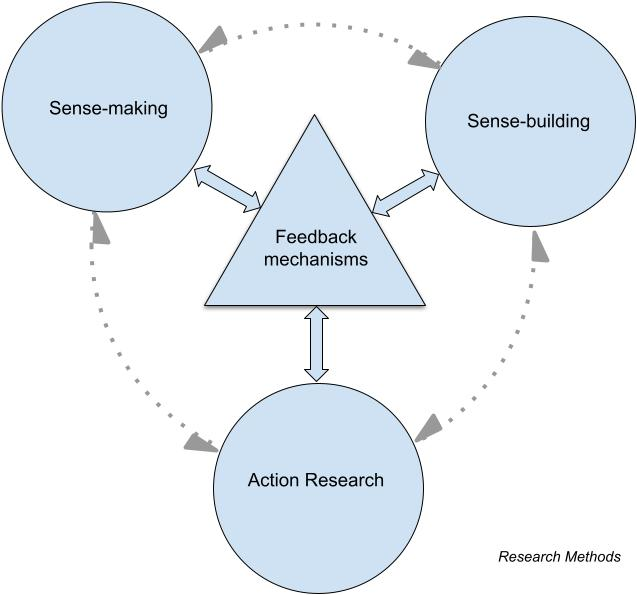
\includegraphics{images/my/categories-of-research-methods-02-aug-2022.jpeg}
    \caption[Categories of research methods]{Categories of research methods \\Source for the figure: {\footnotesize \href{https://docs.google.com/drawings/d/1DpnrvH1ajAKtmcpbJjTWEshdQG_nAIfDS_eAL8obSAQ/edit?usp=sharing}{Google Drawing: Research Methods in PhD}}}
    \label{fig:categories-of-research-methods}
\end{figure}

\subsection{Interviews}~\label{methodology-interviews-topic}
Interviews were qualitative in nature and, as such, primarily open and flexible in their arrangements to facilitate interviewees being able to provide rich experiences and insights as they arose. The case studies included more senior participants and volunteers,  these interviewees have a great deal of autonomy and choose what they are willing to provide including whether they respond at all, (see \sidecite{james2006_credibility_authenticity_and_voice_dilemmas_in_online_interviewing} for a discussion on these aspects). And all participants ultimately had a great deal of freedom in practice in terms of their contributions that formed the basis for aspects of this research and for the use of open and flexible interviews even when interviews were prepared in advance. 

The nature of open and flexible interviews with senior and voluntary participants meant the interviewer needs to be artful in how they design and perform the interviews to maximise the potential value of those interviews. At times in an effective interview 
 questions may be alternate between the interviewer and the interviewee~\sidecite{rapley2001_the_artfulness_of_open_ended_interviewing_etc}.

Many of the case studies overlapped with various lockdowns related to coronavirus~\index{Covid-19} where interviews in person were impractical. That said, e-mail based interviews were already recognised as an established research practice\sidecite{bampton_cowton_2002_the_e_interview}.  And similarly, the use of online interviews, in a similar vein to \sidecite{deakin2014_skype_interviewing_etc}, yet often using other video-conferencing services, formed a key aspect of the research.

The evidence from the interviews was analysed, compared, and filtered to provide representative findings of note. 

\subsection{Categories of research methods}~\label{methodology-categories-of-research-methods}
Figure~\ref{fig:categories-of-research-methods}, on page~\pageref{fig:categories-of-research-methods}, provides a visual overview of the four categories of research methods used to serve this `cognitive ethnography' approach; they include 1) sense-making, 2) sense-building, and 3) evaluation through action research, which were complemented by the fourth category 4) feedback mechanisms to help support and verify the analyses. 

Note: Figure~\ref{fig:categories-of-research-methods} is an over-simplification with clear boundaries between the categories in order to convey the alignment of methods to purposes, and the categories are not discrete.  Some methods include several data sources, and some data sources are analysed using several methods. In practice, individual research methods provided multi-faceted contributions; for instance local app experiments contributed to both sense-building and sense-making. 

Table~\ref{tab:mapping-analysis-to-six-perspectives} identifies the various research methods, groups them in terms of their roles in the research (as illustrated in Figure~\ref{fig:categories-of-research-methods}), and maps them to the six perspectives.  Each of these research methods includes data collection \textit{and} analysis unless otherwise stated.


\begin{table*}
    \small
    \setlength{\tabcolsep}{4pt} %% default is 6pt
    \setlength{\arrayrulewidth}{0.1mm}
    \centering
    \begin{tabular}{l|ccc|ccc}
      & \multicolumn{3}{c|}{\bfseries \small Understand} & \multicolumn{3}{c}{\bfseries \small Improve} \\
      \toprule
         % &\textsubscript{u}Use &\textsubscript{u}Artefacts &\textsubscript{u}Tools &\textsubscript{i}Use &\textsubscript{i}Artefacts &\textsubscript{i}Tools \\
         \multicolumn{1}{r|}{Six perspectives} &\uuse &\uartefacts &\utools &\iuse &\iartefacts &\itools \\ % Thanks to https://tex.stackexchange.com/a/33488/88466
         
        \hline 
        \textbf{Sense-making} & & & & & & \\
        (comprehension and exploration) & & & & & & \\
        Beacon finding and    &S &m &S &m &m &m \\
        Drill-down            &m &m &S &S &m &m \\
        %\tabucline[1pt on 3pt]  \\ % See https://tex.stackexchange.com/a/109301/88466 however here it is terminated prematurely and a bit heavy 
        % Or try https://tex.stackexchange.com/a/229334/88466 or https://tex.stackexchange.com/a/613907/88466 if I've not collapsed these two previous rows soon.
        % Or use a newer latex package, see https://tex.stackexchange.com/a/611494/88466 

        \hline
        \textbf{Sense-building} & & & & & & \\      
        %(Integration and differentiation)    & & & & & & \\        
        (micro-experiments and macro-discoveries) & & & & & & \\
        Local App Experiments   &m &S &S &  &S &S \\
        FOSS Analytics Experiments      &  &  &S &  &  &S \\
        Across Case Comparisons &S &m &S &S &m &m \\        
        
        \hline
        \textbf{Feedback mechanisms} & & & & & & \\
        (triangulation and validation) & & & & & & \\
        Ask The App Devs      &S &m &m &m &m &m \\
        Ask The Tool Devs     &  &  &S &m &m &m \\
        Grey Literature \& Grey Data Analysis       &m &m &S &m &m &  \\
        Code, \& app-binary, Analysis         &m &S &  &m &m &  \\
                
        \hline
        \textbf{Action research} & & & & & & \\
        (embedded intervention)  & & & & & &  \\
        Observation and Analysis &S &S &S &S &S &m \\
        Field Experiment         &m &  &  &S &S &  \\
        Hackathon                &m &m &  &S &S &  \\
        
        \bottomrule
    \end{tabular}
    \caption[Mapping research methods (rows) to the 6 perspectives (columns)]{Mapping research methods (rows) to the 6 perspectives (columns) \\ S = \textbf{S}trong contribution \\ m = \textbf{m}oderate contribution \\FOSS = Free and Open Source Software}
    \label{tab:mapping-analysis-to-six-perspectives}
\end{table*}

`\textbf{Sense-making}'\index{Sense-making} methods were concerned with understanding current practice (as reflected in artefacts, tools, and developers' practices and perspectives -- i.e., perspectives \uartefacts, \utools, and \uuse) and identifying potential improvements in tools and in how analytics are used in app development and maintenance (i.e., perspectives \itools and \iartefacts). The research methods include beacon-finding (see page~\pageref{section-beacon-finding-method}) and drill-down (see page~\pageref{drill-down-research-method}).

Sense-making incorporates an iterative pattern of \textbf{beacon finding} to identify areas of interest within a case, \textbf{drill-down} to investigate one or more beacons, and comparisons both within and across~\footnote{While across-case comparisons are grouped under sense-building, they also help with sense-making.} cases to identify patterns, relationships, counterfactuals~\footnote{\emph{``...relating to or expressing what has not happened or is not the case." Oxford Languages.}}, as some characteristics emerge in contrasts across and between studies. Comparisons were performed iteratively on an ongoing basis (for active apps the values are not constant). These comparisons included comparisons across releases, using different windows of time, on different dates, comparisons with peers, and so on.


`\textbf{Sense-building}'\index{Sense-building} methods build on -- and test -- insights found through sense-making. The research methods included micro-experiments, carried out on local apps (see page~\pageref{local-app-experiments-research-method}), FOSS analytics experiments % COULD-DO Arosha's suggested alternative concepts of white and black box testing of the tools. I'm mulling these over. TBD.} 
(see page~\pageref{foss-contributions-research-methods}), and across-case comparisons (see page~\pageref{across-case-comparisons-research-method}).

Local app experiments\index{Local app experiments} (see page~\pageref{local-app-experiments-research-method}) were used to investigate detail and give insight into the relationships between tools, quality of analytics, and potential impact of analytics use on apps (i.e., perspectives \uartefacts, \utools, \iartefacts, \itools).

Across-case comparisons\index{Across-case comparisons} (see page~\pageref{across-case-comparisons-research-method}) identify macro-discoveries -- that is, they identify characteristics and patterns that were not evident in individual case studies, potential improvements to practice (i.e., perspectives \uuse and \iuse), as well as the influence of the quality of tools in practice (\itools). They can also corroborate and/or challenge findings found in individual cases.


`\textbf{Feedback mechanisms}'\index{Feedback mechanisms} were used to support and verify the other analyses, by comparing observations to other evidence, or by asking developers for clarifications or reflections. Feedback mechanisms were used throughout the research and contributed mainly to the understanding of perspectives associated with (\uuse, \uartefacts, and \utools); nonetheless they were also used frequently when considering improvements (\iuse, \iartefacts, and \itools). 

`\textbf{Action research}'\index{Action research} methods were concerned largely with understanding the use of analytics in context and the evaluation of the effect of improvements in the use of analytics, in terms of adoption into use and app performance (i.e., perspectives \iuse and \iartefacts). It includes three research methods: 1) observation and analysis, 2) field experiment, and 3) hackathon. These are explained on page \pageref{section-action-research-method} onward. 

The research was iterative, moving through sense-making, sense-building and feedback mechanisms repeatedly as new cases were studied or new insights emerged.  The methods and the data sources often also informed several of the six perspectives.  These research methods are introduced in more detail in the sections that follow.

\subsection{Sense-making}\index{Sense-making}
% c.f. https://en.wikipedia.org/wiki/Sensemaking_(information_science)
%1) Identifying patterns (inductive analysis) c.f. grounded theory. 2) 

`Sense-making' focuses on understanding the current practices and identifying potential improvements in practices and tools.  It includes beacon finding (inductive analysis of different forms of data to identify areas of interest) and drilling down (further data collection and analysis to understand those areas of interest in context). Sense-making can include other activities, such as:
 
% NB: I'm not quite sure where to place the following, I might end up moving it or splitting it apart into various sections.
 \begin{itemize}
    \itemsep0em
    \item Collating similar failures.
    \item Ordering and ranking clusters of failures.
    \item Bug identification and localisation: Establishing potentially pertinent patterns in the reports, and characterising when a failure \emph{does and does not} occur are part of this work. Obtaining an identifying definitive boundaries may be impractical, the work is often iterative and exploratory in nature and lossy. 
    \item Bug investigation.
    \item Checking whether there is likely to be sufficient evidence for any triage process.
\end{itemize}

\begin{figure}
    \centering
    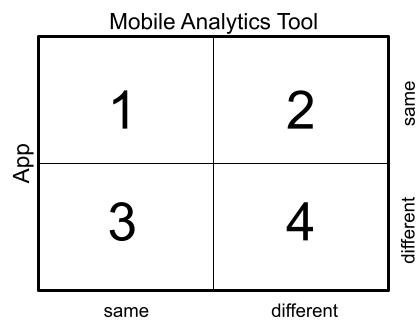
\includegraphics[width=6cm]{images/my/Boston-matrix-app-and-mobile-analytics-tool.jpeg}
    \caption{Boston matrix for app and mobile analytics tool}
    \label{fig:boston-matrix-app-and-mobile-analytics-tool}
\end{figure}

\subsubsection{Beacon-finding}~\label{section-beacon-finding-method}\index{Beacon-finding}

The notion of \textbf{`beacons'} is borrowed from research on program comprehension; for instance by Wiedenbeck, who helped establish the notion of beacons in software development: ~\emph{``In programming, beacons are lines of code which serve as typical indicators of a particular structure or operation''}~\sidecite[][p. 679]{WIEDENBECK1986_beacons_in_computer_program_comprehension}. The work was extended and updated to explicitly consider the effects of beacons in comprehension of source code, for instance in~\sidecite{crosby2002_roles_beacons_play_in_comprehension_etc}.

The notion of beacons was generalised for this research to include indicators in the analytics of something of interest, or something that required attention.  And so `beacon finding' was an inductive process by which significant indicators in the analytics data were identified -- and then used to identify areas of the code base that required further investigation.  Mobile analytics may include source code that calls APIs in the application's source code, however the bulk of the contents that need to be comprehended comes as outputs from the mobile analytics tools, therefore the beacons will differ accordingly. In this research the beacons include: the shape of graphs in mobile analytics report, failure clusters, a method call in stack traces, and so on.

%\marian{Now specify how you spotted beacons... I looked for things on this basis, how I kept track of things, what selection criteria were used and why?}

\textit{Note: In this thesis text in blue boxes are to provide some additional relevant information.}
\begin{kaobox}[frametitle=Beacons in Mobile Analytics]
\section{Beacons in Mobile Analytics}
\textit{This is where I'll gather notes on beacons found in mobile analytics outputs. It may eventually be incorporated into my thesis. For now, it's where raw content and ideas will be collected and later collated.}

Inspirations include:
\begin{itemize}
    \item Scott Barber's work on modelling software performance [testing].
\end{itemize}

Candidates for beacons include (numbered for ease of reference):
\begin{enumerate}
    \item An aggregate increase in error rate
    \item Early adverse trends during a phased release rollout
    \item Correlations with one to a few predetermined factors (e.g. OS release, device model, ...)
    \item 
\end{enumerate}
\end{kaobox}

Beacons emerge in various ways. For instance in reports they include: anomalies within a report, mismatches and inconsistencies between two sibling reports or between a master report and the linked detailed report%~\todo{Arosha, suggested introducing these terms for different types of report when discussing analytics tools in the lit. review. I agree, TBD once the lit. review has been reworked.}
, in the shape of the curve of a graph, in the distribution and groupings of aggregate data, and so on. Similarly, alerts as determined by a mobile analytics service may be considered potential beacons being `promoted' by the mobile analytics reports. 

The most common method of recording potential beacons in this research was using web browser screenshots and/or other mechanisms that preserved information electronically. Some were annotated as part of the beacon-finding and drill-down analysis. Additional notes were written both electronically and/or in physical notebooks. 

Selection criteria included: top ranking results, atypical rates of change, adverse changes to reliability, novel failures particularly for the most recent release, etc. A consistent and overriding criterion was to seek beacons that indicated flaws and failures that could materially and adversely affect the user experience of the app for one or more users of the app.

\subsubsection{Drill-down}~\label{drill-down-research-method}
Beacons identify areas of interest; these need to be investigated further by `drilling down' and examining the underlying information sources. For example:  Is the identified beacon genuinely significant? Does it generalise to other contexts?  What does it signify or relate to in the app and its usage, etc.?  Drill-down starts with the original data sources, but may draw in other data sources to clarify relationships, responses by the developers, etc. 

For Segment 1 of Figure \ref{fig:boston-matrix-app-and-mobile-analytics-tool} (\emph{i.e.} the same app and the same mobile analytics tool) examples include:

\begin{itemize}
    \itemsep0em
    \item Going into greater detail in the current report for a `failure cluster'\index{Failure cluster} to understand its characteristics.
    \item  Investigating in more detail in order to understand the report, the nature of the problem, the causes, and effects. 
\end{itemize}

For Segment 3 (\emph{i.e.} a different app using the same analytics tool) examples include: 

\begin{itemize}
    \item Looking across apps to see if the same and/or similar failures were happening in any of those other apps.
    \item Looking at the characteristics of the failures in the various apps, for instance does a failure happen as often? on the same release of the operating system? on the same device models? and so on.
\end{itemize}

For Segment 2 (\emph{i.e.} the same app using other analytics tools):

\begin{itemize}
    \item Does the same failure appear in all the analytics tools, and if so, are the characteristics similar or do they differ in particular ways?
\end{itemize}

Segment 4 (different apps \emph{and} different tools) did occur sometimes in the case studies, however these are beyond the scope of this research \emph{e.g.} as one of the apps was a web app.

The drill-down may be expanded further using feedback mechanisms, e.g.:
 
\begin{itemize}
\itemsep0em
\item Searching grey data\index{Grey data} and grey literature\index{Grey literature} and cross-referencing of materials.
    \item Asking people: for instance colleagues, the developers of the app, the developers of the mobile analytics tool, \textit{etc}.
    \item Check development artefacts as these may provide relevant and pertinent information and clues.
\end{itemize}

A representative example of using the feedback mechanisms is:

\begin{itemize}
    \item A new release of one of the apps resulted in a five-fold spike in the crash rate for the new release. After drilling-down into both the platform and the in-app analytics, the source code of the network library was reviewed in tandem with searching for similar issues reported on StackOverflow. These helped with identifying the epicentre of the crashes.
    \item Automated tests for the network library were then used as a basis for devising similar tests for the app. These tests reproduced the crash and demonstrated the subsequent changes to the app were effective in fixing the crash.
    \item And when the modified app was released the mobile analytics confirmed the spike had been successfully addressed in the new release.
\end{itemize}

This example served both the research needs and the practical project needs; and it transpires that developers use a similar form of sense-making; this is discussed in \secref{aiu-sensemaking-and-decision-taking-by-developers-section}, starting on page \pageref{aiu-sensemaking-and-decision-taking-by-developers-section}.

\subsection{Sense-building}
Sense-building moves beyond sense-making. Sense-making aims to understand \textit{what is}, while sense-building extends sense-making with direct action and more active research, for example: to devise and run experiments to learn more about the behaviours of mobile analytics, and to seek patterns and generalisations across tools, and case studies. The main methods used for sense-building were local-app experiments, experimentation with \Gls{foss} analytics tools and across-case comparisons. 

\subsubsection{Local-app experiments}~\label{local-app-experiments-research-method} 
\textbf{Local app experiments}\index{Local app experiments} were used to \textit{test the understanding} of the relationships between the usage and the analytics through manipulations of apps and observation of the effects -- hence, the local app experiments were used to test some of the patterns identified in the inductive analysis. They consist of \textit{micro-experiments}\index{Micro experiments} involved creating and developing small mobile apps intended to exercise particular aspects of mobile analytics~\marginnote{Similar to the `invent the future' adage, for example: \href{https://quoteinvestigator.com/2012/09/27/invent-the-future/}{quoteinvestigator.com/2012/09/27/invent-the-future/}}). The inputs to an app were directed in order to determine the outputs from mobile analytics. This was essentially a form of black-box test, where the analytics tool being studied was the system under test \acrfull{sut}\index{System under test (SUT)}. These micro-experiments helped to answer questions and gaps observed as part of sense-making\index{Sense-making}.  In particular, they provided insights into the relationships between tools, quality of analytics, and potential impact of analytics use on apps (i.e., perspectives \uartefacts, \utools, \iartefacts, \itools). 

The apps that were developed as local-app experiments are small mobile apps and not intended for production use. They were developed in order to investigate the relationships between the inputs (such as usage) and the analytics outputs (such as reports) through deliberate manipulation of the inputs and observation of the consequences.  

The local-app experiments allow for tighter control on the usage, \textit{i.e.}, the inputs, in comparison to the unfettered use of real-world mobile apps. They can help surface behaviours and provide for tighter evaluation in the early, pre-launch/pre-production phases. %I can't say feedback as that'd conflate the other use of feedback here in the methodology.
The local app experiments were used to test some of the patterns identified in the inductive `sensemaking' analysis.

Where practical the source code of these apps is made available under a permissive opensource license to facilitate further research by others and in order to facilitate inspection by and feedback from others.

%\akb{Also explain how the results of these experiments connected to other parts of the method? e.g., did they change / add to the sense-making activities?}
The results of the local app experiments helped augment the across-case experiments, particularly in terms of providing additional results to compare with those from the app case studies. They also informed discussions with the app and tool developers. 

\subsubsection{FOSS analytics experiments}~\label{foss-contributions-research-methods}
The research carried out experiments on several \acrshort{foss} analytics tools to gather evidence on how these tools worked. Additionally, these experiments explored the processes used by the relevant \acrshort{foss} projects to accept and adopt contributions that aimed to improve one or more elements of the respective codebase and thereby improve the respective analytics product offering.

As the research had access to the source code of the tools studied, the investigation of how these analytics tools worked can be considered to be a form of white box testing, where simple apps were used as test drivers to exercise the functionality of the analytics components. The exploration of the project processes for adopting changes were more like grey box tests as there was only partial visibility of the dynamics of the relevant project teams. 
The \acrshort{foss} analytics experiments were relatively small in scope and made on an \emph{ad-hoc} rather than a systematic basis~\sidenote{While systematic contributions may be a valid approach to research this topic, it was not core to this research.}.%~\todo{Add table listing analytics tools studied and whether they were subject to black box, white box or grey box testing}

\subsubsection{Across-case comparisons}~\label{across-case-comparisons-research-method}
\textit{Across-case comparisons} were concerned largely with understanding current practice and identifying potential improvements to practice (i.e., perspectives \uuse and \iuse), as well as the influence of the quality of tools in practice (\itools). This method draws on the approach discussed in \sidecite[][pp. 567-569]{seaman1999_qualitative_methods_in_esse}, \textit{e.g.}, to compare pairs of case studies to determine variations and similarities, with the additional considerations of seeking areas of potential improvements based on findings from the various case studies.

Similar to using various software testing techniques to find bugs, making comparisons across the case studies can help to identify more of the behaviours of mobile analytics, their use, and their efficacy. Across-case comparisons can increase the probability of seeing fresh characteristics and establish similarities across cases. The comparisons across case studies help establish norms (which can also be used to identify beacons, and anomalies), patterns (and anti-patterns), variety, and ranges. 

Comparison across cases (\textit{i.e.}, across projects and their mobile apps) helps both researchers and developers, albeit their interests and focus may differ.

\begin{itemize}
    \item \textbf{For developers}: they can compare the reports for their apps with the results others obtain. Doing so may help them identify problems-in-common (shared problems) and fixes-in-common that work for many apps with similar failures. They can also establish norms and the comparisons help provide triangulation and perspective. Some developers also find peer-group comparisons stimulating.
    
    \item \textbf{For researchers}: across case comparisons include `plus one'~\sidecite[][pp. 28-29]{aurini2016_how_to_of_qualitative_research} research that can help uncover emergent behaviour, reinforce existing findings, and so on. The across case comparisons also provide additional microcosms where new findings are discovered in the behaviours of apps, the tools, the development practices, and the efficacy of the use of mobile analytics performed by a wider variety of development teams.
\end{itemize}


The data and the system state for individual apps can help to increase the `coverage criteria' for a mobile analytics tool (which may be considered a system or simply a `box' as in black-box, grey-box, or white-box system)%~\todo{In the planned Tools chapter I can discuss this property of the various Mobile Analytics tools.}. 

We know from a related domain, software testing, that more test cases can increase the detection rate of behaviours. For example, a paper by~\sidecite{briand2007_a_critical_analysis_of_empirical_research_in_software_testing} discusses concepts including the concept of a cost-effectiveness curve and of what the author terms `random variations' and the effect these random variations have on fault detection effectiveness in page 5 of their paper. The set of inputs (\textit{e.g.}, crash reports) into a mobile analytics tool may result in various beacons -- and related data -- appearing in the outputs. By increasing the sets of inputs, particularly from dissimilar apps, there is the potential to increase the appearance of beacons. And the larger volume of beacons across the projects allows for weightier analysis.

A key observation is that detection is not static nor a one-off value; behaviours come and go, particularly in mobile analytics tools where reports are often ephemeral. The value of across-case comparisons increases when the sampling increases to record more of the ephemeral behaviours and outputs.

The nature of this PhD research based on a relatively small number of apps and associated case studies means it is premature to attempt to systematically plot the number of cases against the behaviours that were observed. Instead the focus is on monitoring 
new insights vs. resonance, and how often a new case highlights something that was not noticed in previous ones, even though they were there. % Note I don't have distinct records of when this occurred although it would have done so on many occasions.

\begin{kaobox}[frametitle=Parallels from Software Testing]
\textit{c.f.} Testing and Noticing, by~\textcite{bolton2009_testing_and_noticing}, which discusses noticing (and not noticing) from a software testing perspective.
\end{kaobox}


\subsection{Feedback mechanisms}~\label{methodology-feedback-mechanisms-topic}\index{Feedback mechanisms}
Sense-making and sense-building methods are centred on the research and driven by the researcher's focus and perspective. Unaided -- even if they are productive -- they risk being marginalised and disconnected from the work of others, in particular the work of those who actually develop the apps and the tools. 

This research used four `feedback mechanisms' to validate and challenge the research outputs of sense-making and sense-building:

\begin{itemize}
\itemsep0em
\item ask the app developers
\item ask the tool developers
\item analysis of grey literature and grey data
\item analysis of code
\end{itemize}

The first two (i.e., the mid-study communications with developers) extend understanding of topics emerging from sense-making or sense-building, consistent with Ball and Ormerod's `cognitive ethnography'~\sidecite{ball2000_putting_ethnography_to_work_cognitive_ethnography} and Petre's `targeted observation'~\sidecite[][p.234]{petre2009_insights_from_expert_software_design_practice}, by engaging with the developers who are situated in their actual practice in their real-world microcosm.  For example, the developers can be asked about their experiences, perceptions or reasoning about emergent observations, or to explain particular decisions or practices that have been highlighted by the research. The latter two feedback mechanisms provide comparison to additional data drawn from analysis of existing information (i.e., grey literature\index{Grey literature}, grey data\index{Grey data}, code).  The feedback mechanisms draw on multiple data sources, including some which are independent of the research, hence allowing for comparison/triangulation/colligation -- all with a focus on the research questions.

\subsubsection{Ask the app devs}~\label{section-ask-the-app-devs-research-method}\index{Ask the app developers method}
The developers of the apps are uniquely able to voice their perceptions and thinking on their use, experience, and perceptions of using mobile analytics. They are therefore well placed to provide feedback on their use of mobile analytics and also answer questions about their use of mobile analytics in their development artefacts and their perceptions of the mobile analytics tools.

They are also busy with their challenges related to developing and improving the mobile apps they are responsible for. As Petre notes in~\sidecite{petre2009_insights_from_expert_software_design_practice} experts are willing to try/explore many tools; however they focus on what can help them, and they may discount many aspects of the mobile analytics tools including some of the characteristics and behaviours of interest from a research perspective. Nonetheless from a research perspective it may be useful to learn more about why they have discounted or rejected various aspects of the tools. 

\subsubsection{Ask the tool devs}~\label{section-ask-the-tool-devs-research-method}\index{Ask the tool developers method}
The tool developers understand their mobile analytics tools in depth and many have a unique vantage point to observe how their mobile analytics behaves across a large population of apps. Furthermore they are well placed to design, implement, and release fixes and improvements to their mobile analytics products and services. They understand the rationale of their mobile analytics tools and their user-base. And yet, they do not know everything about how their tools are used or perceived and many are keen to receive feedback and insights accordingly.

The research method entails communicating with knowledgeable, available and interested people who develop (in the broad sense) the relevant mobile analytics tool. The communication may be direct or indirect (for instance via their customer service, via online feedback links, or in the form of contributions to their opensource project). Being able to provide succinct, clear, timely, and relevant communications may increase the chances of engaging in a mutually productive dialogue.

\subsubsection{Grey literature and grey data analysis}~\label{section-grey-literature-and-data-analysis-research-method}\index{Analysis!Grey literature}\index{Analysis!Grey data} %\improvement{So two shades of grey? :)}   

A great deal of grey literature\index{Grey literature} and grey data\index{Grey data}~\sidecite[][pp 219-221]{banks2010_blog_posts_and_tweets_the_next_frontier_for_grey_literature} is available online, covering mobile analytics and to errors, problems related to source code and libraries used in real-world mobile apps. The main sources of relevant grey data include Stack Exchange websites frequented by mobile app developers (particularly \href{https://stackoverflow.com/}{stackoverflow.com}) and GitHub. 

Both Stack Exchange and GitHub provide comprehensive and useful search capabilities which help find relevant content, for instances examples where other development teams have found, understood, and addressed particular crashes in their Android app that also apply to the app in the case study.

\href{https://stackoverflow.com/}{stackoverflow.com} provides facilities that encourage meta-data to be provided by users of the site \textit{e.g.}, tags, votes, accepted answer flag, \textit{etc.}, and their search provides facilities to perform searches that use meta-data as well as free text~\sidecite{stackoverflow2021_search_help}.

The nature of GitHub projects provides some inherent structure which can be utilised when performing searches, for example to search issues and pull requests~\sidenote{\href{https://docs.github.com/en/search-github/searching-on-github/searching-issues-and-pull-requests}{docs.github.com/en/search-github/searching-on-github/searching-issues-and-pull-requests}}. 

\begin{kaobox}[frametitle=Inconsistent terms for searches on GitHub]
Note: GitHub uses the term `qualifier' in the online documentation~\sidecite{github2021_searching_code_github_docs}, and the terms `prefix' and `tag' in their online search page \href{https://github.com/search}{github.com/search} to describe their mechanisms to filter the search results. These mechanisms facilitate structured searches of public projects (and others to which the individual has access).
\end{kaobox}


There are similarities in searching programmer-generated grey literature and the low-ceremony evidence described in \sidecite{scaffidi2007_toawards_a_calculus_of_confidence, scaffidi2007developing} where the sources of evidence include votes received by questions and answers on StackExchange sites and on public issue tracking sites including GitHub and Google. % ADD example of Google  

As an example, \href{https://issuetracker.google.com/issues/128796774}{Issue 128796774} in Google's issue tracker reported stack traces in crash reports were unreadable in Android Vitals after the developer switched to deploying their Android app using App Bundles. Two external developers confirmed the issue, as did the Google engineer. Google claims to have fixed the problem, nonetheless the external developers say it was still occurring months later.

The analysis of this type of issue often includes cross-checking between Stack Overflow and Google's Issue Tracker. Sometimes it also includes reviewing issues on GitHub. Where the issue has been seen in one or more of the app-centric case studies potentially there is enough information from these sources to triage the issue for the respective project.

The grey material\index{Grey material} often provides additional examples and/or corroborates issues found in app-centric case studies.

\subsubsection{Code and app-binary analysis}~\label{section-code-analysis-research-method}   

%\unsure{YY: Can you justify to look at grey literature because the academic literature have not covered the research question?} 

Source code provides a snapshot of raw ingredients used by the development team's build process in order to generate an app. Analysis of the binary provides a snapshot of the final result of the build process of the released app.

Source code often includes at least one build `recipe'~\sidenote{For most Android apps the main build recipe is in the file \texttt{./app/build.gradle}.} so the build can also be evaluated and hopefully reproduced~\footnote{Aside from sensitive ingredients such as signing keys used to digitally sign each binary when it is created.}. The source code's repository augments the source code by recording the historical evolution of the source code.

Code analysis in the context of mobile analytics involves searching for indications of the use of one or more in-app mobile analytics libraries in the project's source code~\sidenote{The \Gls{glossary-exodus-privacy-project} \url{https://reports.exodus-privacy.eu.org/en/}\index{Exodus Privacy Project} is one of several tools that can identify the mobile analytics library in an Android application's binary file.}. The steps performed to identify indicators %c.f. beacons as used in this chapter
of the use of a mobile analytics library include:

\begin{enumerate}
    \itemsep 0em
    \item Examine details in one or more \texttt{gradle} scripts where the analytics are added as a `dependency'; the version of the dependency provides useful meta-data on whether the analytics are actively maintained by the developers. % COULD-DO\textit{e.g.} add code snippet e.g. see https://firebase.google.com/docs/analytics/get-started?platform=android#add-sdk
    \item Examine initialisation of the analytics library in the source code; often this occurs in the Android app's \texttt{Application} class. % Ditto there's an example code snippet at https://firebase.google.com/docs/analytics/get-started?platform=android#add-sdk
    \item Examine \texttt{import} statements in individual source code files that reference the analytics Java package(s).
    \item Search for one or more \textit{wrapper} class files. If these exist, then extend the search for these custom classes in step 3 and 5.
    \item Search for calls to the original and any wrapper mobile analytics API classes. % e.g. based on examples including https://firebase.google.com/docs/analytics/get-started?platform=android#start_logging_events
\end{enumerate}

After the five steps have been completed, the matching lines of source code are then available for analysis. 
%
The analysis can be performed for any snapshot of a codebase \textit{i.e.,} for any commit made to the version control repository. Commands such as \texttt{git blame} provide information of the particular commit where lines of code were last updated and complement analysis of the snapshots.

The application of five steps can be scripted. As an example, in joint research~\sidecite{harty2021_logging_practices_with_mobile_analytics} a mix of manual and scripted steps were applied to enable the analysis of the use of Firebase mobile analytics in all the commits made to 57 opensource Android apps.

A useful confirmatory test to help establish the integrity of an app's codebase is to build the app using the build scripts. There may be additional documentation of the build process available, \textit{e.g.}, in a README file incorporated into the code base.

Analysis of the \textbf{app-binary} was limited to free, public, online services, in particular the Exodus Privacy project and AppBrain. Both of these, for different reasons, analyse the binary file(s) for Android apps on Google Play. The Exodus Privacy project focuses on privacy on behalf of end users and identifies the permissions requested by the app and the trackers embedded in the binary file~\sidenote{\href{https://reports.exodus-privacy.eu.org/en/info/understand/}{reports.exodus-privacy.eu.org/en/info/understand/}}; AppBrain focuses on providing information to app developers~\sidenote{\href{https://www.appbrain.com/info/help/index.html}{www.appbrain.com/info/help/index.html}}. In terms of this research, AppBrain provides statistics on the usage of various libraries across the population of apps in Google Play Store; Exodus Privacy provides details of the trackers used in the apps in the app-centric case studies.


\subsection{Action research}~\label{section-action-research-method}
Avison, Lau, Myers, and Nielsen explain the utility and importance of action research in order to establish the relevance of academic research by trying out theories with practitioners in real situations and in real organisations~\sidecite{avison1999_action_research}. They recommend action research \emph{``because this particular qualitative research method is unique in the way it associates research and practice, so research informs practice and practice informs research synergistically."} [p.94]. Action research is particularly relevant for evaluation, when it \emph{``encourages researchers to experiment through intervention and reflect on their intervention and the implication of their theories."} [p.95]. 

This research applies their recommendation where the research informs the practice of both app developers and the work of the developers of mobile analytics tools. Conversely, the research is enriched through understanding the practices and the potential for the application of mobile analytics to help improve the quality of the work of the app developers. The case studies include examples where the researcher's mode of engagement was:
\begin{enumerate}
    \itemsep0em
    \item a consultant and/or an embedded developer: an active participant integrated into the project team;
    \item a coach: of existing teams of app developers who applied the concepts;
    \item an interviewer: of various development teams to learn of their practices and results;
    \item an analyst/observer: performing static analysis of opensource code repositories~\sidenote{Analysis of proprietary code repositories is also possible, but not practicable for this research owing to confidentiality agreements.}.
\end{enumerate}

All the roles support communications with the project and allow the researcher to ask questions, offer suggestions including issues and/or code contributions, and discuss findings with the developers for their case study. All include at least some observation and analysis. 

The coach and embedded developer roles ended up being fairly similar. They both included organising a hackathon and a field experiment for the the Kiwix\index{Kiwix} and Catrobat\index{Catrobat} projects. The material differences were two-fold: a) the embedded developer role continued for several years, whereas the coach role was for several months, and b) the embedded developer role included contributions to the project's code-base.

The consultant role included engineering leadership, mentoring developers and product owners in learning how they could integrate mobile analytics into their work practices, co-writing automated tests and related code, code reviews, and working with various mobile analytics tools throughout the assignment. (Table \ref{tab:app-centric-studies-research-perspective} maps the roles to the app centric case studies.)

\newthought{Engagement:}
The action research was preceded by discussions with the project team (and its organisation) to determine: 

\begin{itemize}
\item what research would be viable and productive; 
\item the role of the researcher; 
\item the depth, scope, range, and duration of the case study; 
\item concerns and constraints that needed to be addressed to protect all the stakeholders involved~\sidenote{The stakeholders may extend beyond the primary participants; for instance, the end users could potentially be stakeholders in what happens during the case study.} while also maintaining the integrity of the research;
\item intellectual property rights, copyright, confidentiality, non-disclosure agreements, and so on~\sidenote{Note: some researchers may be introduced to these together with the ethical aspects under the term LSEPI, discussed in ~\cite{brooke2018__becoming_professional_a_university_perspective}}.
\end{itemize}

The decisions were made mutually by the parties involved. Generally, the project's team and its organisation set the limits and constraints. As \sidecite[][p.324]{barroca_2018_bridging_the_gap} notes, timeliness and relevance are vital to industry partners, while they also want to guard against the research being too intrusive or too demanding of their time or other resources. Therefore, the research needs to offer something of sufficient value, relevance, and timeliness to the project team and its organisation. For example, if they are aware their projects have excessively-high error rates %(for instance if they are aware of these via their mobile analytics reports)
, they may have the motivation to participate in the research in the hope of materially reducing the error rates, and furthermore they may seek an intervention in the guise of action research in order to achieve reductions in any excessively-high error rates.  As the projects generally already have at least one form of mobile analytics, the incremental cost is low in terms of tooling.


\newthought{Wrap-up: }
The wrap-up of a case study included various actions such as safeguarding and archiving evidence; redacting personal details or anonymizing communications with the stakeholders; unsubscribing from services provided for a given case study~\sidenote{Note: the project team may control the researcher's access to various systems and development artefacts, and perform their own equivalent of a wrap-up.}; reviewing findings, analysis, and conclusions with the development teams (and with their organisation); preparing what is appropriate to publish in terms of evidence, and so on. This stage also provided an opportune period for retrospectives of the case study \textit{and} for the research methods and outcomes, while the case study was still topical. 

\subsubsection{Observation and analysis}~\label{section-observation-research-method}
Observation is combined with analysis, both contemporaneous and \emph{post-hoc}.   Findings were presented to the project and development team, in order to: 1) provide value for the team members who were willing to contribute their time and who provided access to their analytics and other artefacts, and 2) encourage scrutiny and validation of the findings and observations.

In this research, observation included either or both development artefacts and analytics artefacts. One example is to observe the outputs from mobile analytics tools (the analytics artefacts) and what the developers do with these subsequently. 

The analysis focused on ways the observations might usefully help the project in terms of improving their development practices and/or their artefacts.

\newthought{Contemporaneous analysis:}
The nature of working with live mobile analytics data and real-world projects means there are likely to be important events that need to be found and processed rapidly in order to preserve their value in terms of the case study. Therefore, one of the success factors in terms of the research is to practice continuous, ongoing, low latency, and iterative analysis, verification, course correction, efficacious communications -- where it is viable to do so~\sidenote{In other words, there are four key tasks: analysis, verification, course correction, and efficacious communications. All of these need to be performed on a continuous, iterative, and ongoing basis. Keep latency in the work to a minimum in order to increase the value of the results and the effects.}. The viability is governed by various factors, including: the working relationships with the project team set in the context of their working practices, research access to the various systems, and the characteristics of the event being reported via the mobile analytics tool(s). 

\newthought{Post-hoc analysis:}
\emph{Post-hoc} analysis is more research-oriented; in contrast analysis during the active case study is often more project-oriented. During the active case studies, there is a need to deal effectively with ephemeral events, data, actions, \textit{etc.} on an opportunistic, often sporadic, basis; there is potentially a bias toward tactical findings and outcomes. From a research perspective, the active case study may appear messy, chaotic, and yet incomplete. The \textit{post-hoc} stage provides the complementary opportunity for a more reflective, objective, and strategic perspective. It can help reduce inadvertent bias in the more immediate tactical work by seeking counterfactuals, alternatives, and/or mistakes and flaws.

By the \emph{post-hoc} analysis stage, the active engagement with the project has tapered off, although in some cases additional updates may be available; e.g., some projects have provided ongoing access to mobile analytics and/or updates from the project team. Nonetheless, for the most part the evidence has been harvested, and any active interventions have ceased. The  \emph{post-hoc} analysis of collected records, actions, and results seeks to identify patterns in and across case studies, as well as to identify contradictory evidence,  misconceptions, and potential omissions.  Applying the six perspectives (illustrated in Figure~\ref{fig:six-perspectives-in-the-methodology}) help to categorise and group various findings in the \emph{post-hoc} analysis. 

Conclusions, together with their supporting findings and their respective sources, were verified with the project team when feasible. 

\newthought{Analysis of findings:}
Conceptually, the findings were analysed systematically, and the findings were first analysed at a granular (low) level; these were then aggregated into higher level themes. Both the lower- and higher-level themes were counted to establish their relative frequency in the findings. 
To support the analysis, a spreadsheet was used that incorporates named ranges and formulae to reduce manual errors and make the analysis easier to scale and revise as any new findings emerged. Details on how the thematic analysis was performed are available in the \href{appendix-thematic-analysis}{\nameref{appendix-thematic-analysis}} appendix.

The approach I used was similar to the six-phase approach described in ~\sidecite{braun2012_thematic_analysis}, %They provide a six phase process, which I would have used as-is if I had known about their approach during my analysis; nonetheless, my approach was similar and corroborates theirs 
albeit I used themes at both the lower and higher level analysis, along the lines of~\sidecite[][pp. 280-281]{cruzes2011_recommended_steps_for_thematic_analysis_in_software_engineering}. Visual modelling helped organise the themes and their relationships, as per [p. 280] in the same research. The visual models, in the form of Ishikawa (fishbone) diagrams were reviewed with several academic colleagues and refined iteratively together with suitable revisions to the various themes.

\subsubsection{Field experiment}~\label{section-field-experiment-method}\index{Field experiment}
In this research, field experiments used real-world apps and their core code repositories. They were not as rigorous as controlled experiments due to the nature of the development teams and their priorities. Nonetheless, they included a control app and an experiment app;  experiments were performed on the experiment app and mobile analytics results compared for both these apps. They are also ecologically valid, ~\sidecite[][p.126]{Ko2015_a_practical_guide_to_controlled_experiments_of_sw_eng_tools_with_human_participants}, as they were situated in real-world challenges found in their core mobile apps.

The approach described in~\sidecite{Ko2015_a_practical_guide_to_controlled_experiments_of_sw_eng_tools_with_human_participants} was not suitable for several reasons~\sidenote{This form of research may be useful and also viable for large, funded research groups and/or for organisations such as the larger mobile analytics tool providers, particularly Google. That said, Google in particular has access to such a vast range of data about the use of their mobile analytics tools they may not need or want to perform controlled experiments of the form discussed in this research.}. 
%
My research didn't have the opportunity to compare two tools quantitatively, nor was it practical to perform quantitative research experiments, as none of the projects was interested in the complexity and demands of the type of controlled experiments illustrated in their research. Therefore, the field experiments were designed to suit the specific opportunities provided by the respective projects as follows:
\begin{itemize}
    \item Hackathons were used to initiate the field experiments for the opensource projects. These were attractive to the development teams, partly as they were for a distinct period when the team was able to meet and enjoy the experience of collaborating.
    \item Both the opensource projects had multiple apps, including one that had the worst reliability of their apps (as measured by mobile analytics). The project leads saw value in helping arrange and support the hackathons. They also had apps which were suitable to act as the control for their hackathon. 
\end{itemize}

\subsubsection{Hackathon}~\label{section-hackathon-research-method}
This research method applied the concepts of software development hackathons\index{Hackathon} and added the use of mobile analytics tools as a source of information related to issues in the behaviour (\emph{i.e.}, failure data) of one of more of that team's mobile apps.

In the terminology of \sidecite[][pp. 1-3]{drouhard2016_typology_of_hackathon_events} (as used in ~\sidecite[][p.3]{medina2020_what_do_we_know_about_hackathons_etc_a_SLR}), the hackathons were 
\emph{communal} as the participants were part of common development communities (as developers for the opensource apps they contributed to); \emph{contributive} as there were common concerns about the issues the hackathons were intended to address with a strong desire for impact; and \emph{catalytic} as one of the aims was to demonstrate a new approach to the use of a dataset (mobile analytics reports) and technology (mobile analytics tools).  

No rewards were offered to participants beyond being at the respective hackathon\index{Hackathon} and participating. ~\sidecite[][p.5]{briscoe2014_digital_innovation_the_hackathon_phenomenon} termed these `Single-Application' hackathons. The participants were current members of the respective development team.  The hackathons included the researcher and a highly-experienced leader and contributor in previous hackathons. They prepared much of the hackathons together; and in one case (PocketCode) co-led the hackathon. The app, topic, and focus were both selected as part of the preparations. The work during the hackathon was determined by the participants, with guidance and suggestions from the organisers.

% https://hackathon-planning-kit.org/ 

The outcomes of the hackathons\index{Hackathon} included bug reports, and code changes \emph{i.e.} fixes intended to address some of the bugs found in the respective hackathon. Both the bug reports and the code changes were analysed over a period of several months to observe the effects of each hackathon. The mobile analytics reports were also monitored as new releases of the respective apps were launched to observe the effects of the code changes.

\subsection{Summary of the analytics-centric methodology}~\label{analytics-centric-methodology-section}

The research needed to be grounded in real-world projects and with real-world app development teams; accordingly the methodology incorporates a mutually-beneficial, symbiotic, bi-directional connection where the iterative research is evaluated with and through these real-world projects and teams. 

The analytics-centric methodology grounded in case studies corresponds in principle to the structure and premises of grounded theory~\sidecite{corbin2014_basics_of_qualitative_research_4th_edition} where patterns are induced, data iterated to see if categories are appropriate, and identifying patterns with comparisons with other data sets for checks and balances. Although the research includes a variety of apps, development teams, and mobile analytics tools, the practical limitations of PhD research compared to the vast volumes of apps, mobile analytics tools, and so on means the research and therefore the results cannot be definitive. The research will not reach saturation in terms of determining the transition point where additional cases wouldn't contribute new insights.


\section{Introducing the case studies}~\label{section-introducing-the-case-studies}
All the case studies involved application of sense-making, sense-building and feedback mechanisms. There are two broad categories of case study: app-centric and tool-centric. 

Each app-centric case study is centred around a single codebase, that codebase may be used in one app or in several, and the organisation may have additional code bases and associated apps. In the Catrobat\index{Catrobat} case study the additional app and codebase provide a useful contrast to the primary one in the case study.

The tool-centric case studies are centred on a single mobile analytics tool. Some of the tool-centric case studies emerged from the app-centric case studies, others emerged from mini-experiments or from grey materials.

\subsection{Introducing the app-centric case studies}~\label{methodology-introducing-the-app-centric-case-studies-section}
For the app-centric case studies in this research, every project included at least one actively-used Android app in Google Play\sidenote{By having an active app in Google Play they will also have access to the Google Play Console\index{Google Play Console} with its dashboard, Android Vitals, release tools, and other related reports. Therefore they will \emph{de-facto} have at least one source of analytics, collected by the Google Android platform.}. The case studies range in the richness of their contributions to the research; Table~\ref{tab:app-centric-studies-research-perspective} provides the research context for each of the seven app-centric case studies. The table has four groupings, these are for the four main research methods used in these case studies. The first grouping (and main research method) is for the interview-centric case studies, those without a planned intervention. The other three research methods all involve at least one planned intervention.

As Table~\ref{tab:app-centric-studies-research-perspective} indicates, four project teams were interviewed to provide the developers' perspectives on their use of various mobile analytics tools. Two of these (LocalHalo\index{LocalHalo} and \acrshort{gtaf}\index{GTAF}) provided real-time access to at least one of these tools. GTAF also provided access to their bug tracking system which records issues they find using mobile analytics.

During this research I was already working as part of a development team for the Kiwix\index{Kiwix} project. The other cases were accessed through personal recommendation; two were via academia (Catrobat\index{Catrobat} and \acrlong{gtaf}) and the rest via software developers in industry.


\begin{table*}
    \centering
    \footnotesize
    \begin{tabular}{clllp{3.3cm}p{3.3cm}}\toprule
    & Case Study                 & Main Research Role &  Main Research Method   & Research Opportunities             & Research Purpose \\
    \arrayrulecolor{blue!70}\midrule
    \multirow{5}{*}{\large {\rotatebox[origin=r]{90}{Interviews}}} & GTAF                       & Interviewer        & Ask the app devs & Additional perspective & Exploring the long tail \\
    & LocalHalo                  & Interviewer        & Ask the app devs & Additional technologies & Hybrid Programming and tools \\
    & Moodspace                  & Interviewer        & Ask the app devs & Small startup &Bootstrap view \\
    & Moonpig                    & Interviewer        & Ask the app devs & Leading edge view & Mature, innovative, vanguard dev. practices \\
    & Smartnavi                  & Interviewer        & Ask the app devs & Opensource codebase that incorporates Crash reporting and Firebase Analytics & Compare our analysis of their source code with the developer's intentions \\
    \arrayrulecolor{blue!70}\midrule
    \multirow{6}{*}{\large \rotatebox[origin=r]{90}{Interventions}} & Kiwix (Kiwix app)          & Embedded           & Field-experiment   & The proof-of-concept      & The treatment \\
    & Kiwix (WikiMed (EN))       & Analyst/Observer   &                    & Control for the above app & The control  \\
    & Kiwix (Custom apps)        & Analyst/Observer   &                    & Evaluate scalability      & \textit{pico} generalisation \\
    \arrayrulecolor{blue!20}\cmidrule{2-6}
    & Catrobat (PocketCode)      & Coach              & Hackathon   & Fabric Crashlytics        & Compare Mobile Analytics with Clean Code \\
    & Catrobat (PocketPaint)     & Analyst/Observer   &                    & Establish baseline        & The control  \\
     \cmidrule{2-6}
    & C1                         & Consultant         & Hybrid/Mixed & Large scale, complex, commercial & Mission-critical view \\
    \arrayrulecolor{black}\bottomrule
    \end{tabular}
    \caption{App-centric cases: the research perspective}
    \label{tab:app-centric-studies-research-perspective}
\end{table*}

Three project teams were subject to interventions. Of these, both Kiwix\index{Kiwix} and Catrobat\index{Catrobat} develop and work as opensource projects where access to their code, to their issue tracking, and to other aspects of their projects are public. They both also provided access to their mobile analytics tools. The last of these case studies, C1\index{C1}, is based on a mission-critical commercial product where a similar approach to applying mobile analytics was applied for the Android app element of the product.

%%%%% Marian, all, please help me integrate and prune the following material (relocated from the apps and their artefacts chapter).
\newthought{Sources of `truth'}
In terms of the app-centric case studies there are several sources of `truth' in terms of the use of mobile analytics. These include:
\begin{itemize}
    \itemsep0em
    \item The developers: including what they say they do, and how they used mobile analytics.
    \item The source code, including the build scripts and relevant configuration files. The source code + the build process generates one or more application binaries, and they may also generate and run various automated tests that exercise the app and/or the mobile analytics SDK(s).
    \item The app binary: encapsulates and packages the software that is intended to run on end-user devices. 
\end{itemize}

This research included interviewing some app developers and working with others to learn about their perceptions of using mobile analytics and the artefacts they created in the process.

Whenever the source code was available it was studied to learn how mobile analytics had a) been integrated b) been used to effect changes in the source code. 

The Exodus Privacy project~\sidenote{https://reports.exodus-privacy.eu.org/en/} was used to detect whether the app binary included the appropriate mobile analytics \Glspl{sdk}.

% \isabel{Do you need to put in a sentence just splitting "truth" into facts, perceptions, opinions (and indeed attempts to deceive).? I read something recently (but where?) about the difference between honest and truthful = honest being what you genuinely believe, and truthful being the facts - Is that where you are going with this? What the developers say they do, versus what they actually do...?}


\subsection{Introducing the tool-centric case studies}~\label{methodology-introducing-the-tool-centric-case-studies-section}

The app-centric cases were complemented by empirical studies with several providers of mobile analytics tools where there was mutual interest in exploratory field studies; Table~\ref{tab:tool-centric-studies-research-perspective} provides the research context for the tool-centric case studies. They entries are grouped by the main research method.

The tool-centric studies range from those that were part of an app-centric case study (the first four listed in Table~\ref{tab:tool-centric-studies-research-perspective} \textit{i.e.}, Fabric Crashlytics\index{Crashlytics!Fabric}, Microsoft App Centre\index{App Center}, Sentry\index{Sentry}, and Google Play Console\index{Google Play Console} with Android Vitals\index{Android Vitals}). Of these the Google Engineering team choose to engage further with the research and the findings based on the initial findings regarding behaviours and flaws in Android Vitals and Google Play Console.

Iteratively (who sought out the researcher, learned about the research, and was happy to share their tools and some of its commercial research), and several mobile analytics providers who provide at least some of their material as opensource. 

Shortly after Iteratively was acquired by Amplitude, the Iteratively SDK was incorporated into an updated version of one of the small local app experiments. In effect it was an informal, early-experience program (\acrshort{ieep}) which continued during the post-acquisition integration of Iteratively's product into Amplitude and the migration of the mobile analytics account.

Finally some minor contributions to two mobile analytics tools that include opensource elements which are not listed in this table (PostHog and Sentry). These minor contributions are presented in \secref{section-contributions-to-opensource-mobile-analytics-projects}, starting on page \pageref{section-contributions-to-opensource-mobile-analytics-projects}.


\begin{table*}
    \centering
    %\tabcolsep=0.06cm
    %\tiny
    \footnotesize
    \begin{tabular}{p{3.2cm}llp{3.3cm}p{3.3cm}}
    \toprule
    Case Study              & Role of Researcher    &  Main Research Method & Research Opportunities             & Research Purpose \\
    \midrule
    Firebase Analytics      & Interviewer           & Ask the app devs      & Insights into maintaining a reliable app  & Obtain expert user's view of the most popular mobile analytics tool \\
    \arrayrulecolor{blue!20}\midrule
    
    Fabric Crashlytics      & Analyst/Observer      & Sense-making          & Compare 2 Google Analytics tools  & Triangulation \\   Microsoft App Centre    & Analyst/Observer      & Sense-making         & Crash \& Error analytics          & Blue-chip alternative \\
    Sentry                  & Analyst/Observer      & Sense-making          & Mobile analytics for React Mobile cross-platform apps    & Increase variety and coverage of tools \\
    \arrayrulecolor{blue!20}\midrule

    Google Play Console with Android Vitals & Analyst/Observer  & Ask the tool devs & Mutual symbiotic cross-pollination & Learn about the providers' perspectives \\
    Iteratively             & Consultant            & Ask the tool devs & `Behind the curtain' & Discover state of the art approach to improving the rigour of mobile analytics \\
    Iteratively->Amplitude  & Interviewer \& IEEP & Ask the tool devs & Explore state of the art novel tool & Insights into \itools \\
    \arrayrulecolor{black}\bottomrule
    \end{tabular}
    \caption[Tool-centric cases: the research perspective]{Tool-centric cases: the research perspective \\ {\footnotesize IEEP = Informal Early Experience Program}}
    \label{tab:tool-centric-studies-research-perspective}
\end{table*}


\section{Ethical considerations}~\label{methodology-ethical-considerations-section}
The research was informed by both the researcher's professional experience as a software engineering practitioner, and professional codes of practice. Where appropriate ethics approval was obtained from the Open University's Human Research Ethics Committee (HREC).

During the research, I was a member of three relevant professional bodies: the British Computer Society (BCS), the IEEE, and the ACM, and worked to abide by their respective codes of conduct~\sidecite{bcs_code_of_conduct_2021, ieee_and_acm_code_1999on}.

The ethical considerations implemented during this research can be described using the core concepts presented by Singer and Vinson, namely: \emph{``informed consent, scientific value, beneficence and confidentiality"}~\sidecite[][p.1178]{singer2002_ethical_issues_in_empirical_studies_of_software_engineering}. 

\newthought{Informed consent:}
Consent was obtained from the development team leaders and development team members who participated; and consent was also obtained from their respective organisation as appropriate. In every case they were explicitly aware of the research from the outset of discussions.  Consent was obtained during the engagement discussions, and in some cases had to be extended during later phases, e.g., if the scope of the study increased and/or additional mobile analytics tools were introduced.

\emph{De-facto} consent was also given in terms of the access provided to the tools and artefacts that teams and their organisations provide during the case study. They may also place constraints on aspects of the use of the materials obtained, \emph{i.e.}, consent may be fine-grained and also context dependent.

Additionally, consent was obtained from the app development teams to share findings with the mobile analytics development teams and vice-versa as and where appropriate. This was not applicable in all the cases.

\newthought{Scientific value:}
The importance and relevance of seeking ways to improve the quality of mobile apps and the processes used when developing those apps have been confirmed from multiple sources, including academia and industry.%\todo{Cross-link with the related work chapter.} 
The importance of mobile analytics is evidenced by the practices of app developers who include mobile analytics in over 75\% of all Android apps in Google Play, and by the ongoing development of a multitude of mobile analytics tools and related services. This research aims to contribute to knowledge about the practices, the tools, and the outcomes of using mobile analytics tools as part of development practices. 

\newthought{Beneficence:}
Beneficence aims to maximise the overall benefits for all the stakeholders and harm none. This includes the people who participate in the development teams, their organisations (where applicable), and the end users of their mobile app(s).  The different beneficiaries of the research can be summarised as follows: (1) app developers by helping them make effective use of mobile analytics; (2) organisations involved by helping improve the quality of their apps; (3) analytics tool developers by providing insights into tool use and potential improvements; and (4) end-users by potentially improving the app's performance and reliability downstream.

\newthought{Confidentiality:}
The confidentiality of the participants and also of the information provided and/or gleaned during the case study was protected unless a) the work is in the public domain, or b) permission was granted to make the information public \textit{e.g.}, as part of this research.
As the apps run on end-users' mobile devices, the risks of the data collection and the use of that data were also considered throughout the research. In particular, although some of the apps of the projects do contain \href{glossary-pii}{PII}, no PII was collected or analysed in the mobile analytics from a research perspective.

\newthought{Agency of participants and their organisations:}
`Agency' is the concept that the organisations and the relevant people were free to choose whether they wished to participate in the research, and if so potentially the nature of their involvement and/or the nature of the research. 

Some candidate projects declined to participate in the research on behalf of their project or organisation for various reasons. A common reason was lack of time on their part, another was that some candidate projects perceived the research would not be acceptable to their organisation, for instance owing to confidentiality or business risk. The participating projects chose their model of engagement, which meant the researcher needed to negotiate the modes of engagement to balance ways of working necessitated by the research with the industry practices in domain of mobile app development.


\section{Validity and rigour}~\label{methodology-threats-to-validity-section}
This section discusses the validity and rigour of the research in terms of the methods adopted for data collection and analysis. It complements the later reflections on threats to validity that are presented in the Discussion chapter (see page \pageref{discussion-threats-to-validity-section}).

The use of case studies to explore how analytics affect mobile app development processes and the apps themselves results in a natural trade-off between the internal and external%\todo{Revisit once I've got my copy of \textcite{corbin2014_basics_of_qualitative_research_4th_edition}}
(including ecological) validity of the research. Because the research is being conducted in the context of mobile application development projects, with limited ability to control for external factors, the internal validity of the overall findings is low. However, the aim of the research is not to \textit{prove} hypotheses about the causal  relationships between mobile analytics and the quality of the software developed.  Instead it is to explore systematically the phenomena relating to the effect of mobile analytics on development processes and artefacts, and use these findings to support the formulation of hypotheses for further study. In order to ensure that such exploration is grounded in real-world experiences, it was considered appropriate to give priority to  external (and ecological) validity over internal validity.

The approach adopted to maximise the rigour of the research is to ensure that the methods chosen for data collection and analysis are repeatable. While the specific case studies covered in the research were selected opportunistically, the methods used to collect data and analyse it can be carried out by other researchers. The remainder of this section provides some further details of how the research design supports external validity and repeatability.

\textbf{External validity}: was high for both the app and the tool case studies. While it was not practical or viable to control all the factors, the use of control apps, and tracking the changes made to the source code provided probable causation in terms of connecting cause and effect in terms of increases in the stability of the apps being subject to the interventions.

At least some of the results from the micro-experiments also led to subsequent outcomes in the real-world apps and tools. These outcomes help validate the external validity of these more controlled experiments. 

At least two of the software utilities that were developed as part of this research have been used by other projects, \myindex{Vitals Scraper} was used at \myindex{Moonpig} and \myindex{AndroidCrashDummy} was enhanced and used by a corporation (details of whom are covered by private communications). These help provide some indication the software developed as part of this research are reproducible. Also, a set of artefacts generated by Vitals Scraper have been published and made available to the research community. 

 It is also noteworthy that all the case studies  are real-world projects with real-world engineering desires to apply mobile analytics, \emph{i.e., ``illustrating a tool’s benefits (or lack thereof) on a real software engineering activity taken from practice"}~\sidecite[][p.126]{Ko2015_a_practical_guide_to_controlled_experiments_of_sw_eng_tools_with_human_participants}. When considered together with fact that the case studies cover a variety mobile application development contexts, this supports the \emph{ecological validity} of the research.

\textbf{Repeatability}:
As mentioned here and elsewhere in the dissertation, the software developed as part of this research has been released under a permissive opensource license to encourage and facilitate further research, and a set of the outputs generated by \myindex{Vitals Scraper} have been preserved and made available.


\section{Chapter summary}~\label{methodology-summary-section}
The methodology has been chosen to maximise the viability of answering the primary research question in real-world projects and contexts where access to the tools is granted by project teams and their respective organisations, and where the development teams actively engage and support the case studies.

The methodology also accommodates complementary research that augments the case studies, for instance with the analysis of various opensource Android codebases) introduced in \secref{section-sourcecode-analysis-to-augment-app-centric-case-studies}.

The six perspectives inform the methodology by helping ensure that combinations the various methods address the three key objects of analysis and also address the temporal dimension of determining what \textit{is} and what \textit{could be}.

The Discussion chapter includes various reflections on the methodology, in \secref{discussion-on-methodology-and-case-study-procedure} starting on page \pageref{discussion-on-methodology-and-case-study-procedure}.

The next chapter introduces each of the case studies.